\documentclass[a4paper,11pt]{article}
%\usepackage[utf8]{inputenc}

\usepackage{amsmath, amsfonts, amsthm, bbm}
\usepackage{graphicx} 
\usepackage{bmpsize}
\usepackage{tikz}
\usetikzlibrary{arrows,calc,patterns,decorations.markings,decorations.pathreplacing,plotmarks,shapes.arrows,decorations.pathmorphing,backgrounds}
\tikzset{snake it/.style={decorate, decoration=snake}}
\usepackage[all]{xy}

\usepackage{bm}
\usepackage{hyperref}
\usepackage{float}
\usepackage{titling}
\usepackage{caption}
\usepackage{subcaption}

\numberwithin{equation}{section}
\theoremstyle{definition}
\newtheorem{definition}{Definition}
\newtheorem{theorem}{Theorem}
\newtheorem{lemma}{Lemma}
\newtheorem{prop}{Proposition}
\newcommand{\dbyd}[2]{\frac{\partial #1}{\partial #2}}
\newcommand{\vsig}{{\bm{\sigma}}}
\newcommand{\R}{\mathbb{R}}
\newcommand{\uone}{{u_1}}
\newcommand{\utwo}{{u_2}}
\newcommand{\chii}{\chi^{\vphantom{|}}}
\newcommand{\Tr}{\mathrm{Tr}}
\newcommand{\cH}{{\cal H}}
\newcommand{\NS}{{{\scriptstyle N\!S}}}
\newcommand{\tq}{{\tilde q}}


\setlength{\parindent}{0pt}
\setlength{\parskip}{3pt}

\title{A Treatise on Electricity and Magnetism}
\author{Author: James Clerk Maxwell \\
Student number: 6100001\\
\\ Supervisor: Prof Michael Faraday FRS \\ Module Code: 7ccmtp50}
\date{1861/62}

\usepackage{geometry}
\geometry{a4paper, left=25mm, right=25mm, top=30mm, bottom=25mm}

\renewcommand{\baselinestretch}{1.2}

\begin{document}


\clearpage\maketitle
\thispagestyle{empty}
\begin{figure}[H]
    \centering
    \vspace{100mm}
    
\includegraphics[width=0.2\columnwidth]{kcl_logo.png}
\end{figure}

\newpage

\begin{abstract}

In this paper we shall rigorously define a set of $4$ equations
describing the electro-magnetic interactions. We argue that in the
existing literature there is some confusion about the displacement
current. We demonstrate that this extra term is needed in order for
the equations to enjoy the Lorentz symmetry. 

We also speculate about the constancy of speed of light but our
discussion is not conclusive and requires further investigation. 

\end{abstract}
\newpage

\tableofcontents

\newpage
\section{Introduction}
\label{intro}

This \LaTeX\ project template is just one way you might choose to
present your project. It is based, with some small modifications, on
the template written by Prof Nikolay Gromov for the Mathematics 3rd year
project. 

It has all the essential elements for the MSc project - a title page, an
abstract, an introduction, the main body of the text, a conclusions
section and a bibliography. 
It also include optional sections such as acknowledgements, an
appendix and a sample of Mathematica code. 

Please feel free to adopt and adapt this template. there is a vast
amount of information on \LaTeX\ available online with just a few
links and selected guides on the KEATS web page.

If you want to see how something in this file is done, just look at the
source code!

\section{Another Section} 
\label{sec:2}

Informally, we can think of minimal surfaces as minimising area at
each point of the surface. By this we mean given a point on a minimal
surface if we restrict our surface to a small open neighbourhood
around this point, and consider its boundary, then any small
deformation of this restricted region keeping the boundary invariant
results in an increase of surface area. 

In this section we shall define the notations of a surface and various
other tools and properties required to study minimal surfaces,
resulting in a rigorous definition of a minimal surface. 

\subsection{A subsection title}
\label{mike}

\begin{definition}[Surface] This is one way to write definitions.
A \emph{surface} is a mapping from an open subset of the Euclidean
plane, i.e. $D \subset \R^2 $, into a subset of Euclidean space, $
\R^3 $. We shall use $\vsig(\uone, \utwo)$ as our surface map where $\vsig :
D \rightarrow \R^3 $. That is to say $\vsig$ is a function which maps
the point $(\uone, \utwo) \in \R^2$ to $\vsig(\uone,\utwo) \in \R^3$. 
\end{definition}

Here are some equations

\begin{align}
  g_{ij} 
= \dbyd{\vsig}{u_i} \cdot \dbyd{\vsig}{u_j}
\;, 
 \quad i, j = 1, 2\;. 
\label{fund1}
\end{align}
Some examples of equations:


\begin{equation} 
f(x)=(x+a)(x+b)
\end{equation}

\begin{equation} \label{eq:someequation}
6^2 - 5 = 36-5 = 31
\end{equation}

This references equation \ref{eq:someequation} using the \verb#\ref# command


\begin{equation} \label{eq:erl}
a = bq + r
\end{equation}

where \eqref{eq:erl} is true if $a$ and $b$ are integers with $b \neq
c$. Here the equation was referenced using the \verb#\eqref# command

 \begin{equation}
L' = {L}{\sqrt{1-\frac{v^2}{c^2}}}
\end{equation}

Maxwell's equations:
\begin{align}
B'&=-\nabla \times E,\\
E'&=\nabla \times B - 4\pi j,
\end{align}

\[
A \overset{!}{=} B; A \stackrel{!}{=} B
\]

\[
\lim_{x\to 0}{\frac{e^x-1}{2x}}
\overset{\left[\frac{0}{0}\right]}{\underset{\mathrm{H}}{=}}
\lim_{x\to 0}{\frac{e^x}{2}}={\frac{1}{2}}
\]

\subsection{A subsection on inserting pictures}

You can include pictures from various formats
\begin{figure}[H]
	\centering
	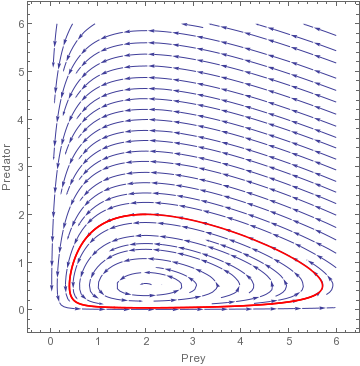
\includegraphics[width=7cm]{totalplot.png}
	\caption{You can prepare your picture in an external editor
          (or export it from for example from Mathematica, as above, or other software)}
	\label{fig:lotka-volterra} 
\end{figure}

You can also use various packages to draw your own - this is an
example using {\em tikz}. There is a good manual online and it is very
powerful, if you want to use its many features.
\begin{figure}[H]
{
\begin{center}
\begin{tikzpicture}
	\pgfmathsetmacro{\hshift}{4}
	\pgfmathsetmacro{\vshift}{2}

	% left part
	\draw (2-\hshift,0) -- (2-\hshift,4);
	\node[left,text height=1ex,text depth=.25ex] at (1.8-\hshift,3.5) {Ising Model};
	\node[right,text height=1ex,text depth=.25ex] at (2.2-\hshift,3.5) {Free fermion};
	\node[above] at (2-\hshift,4) {$I$};
	
	\node[circle,fill,inner sep=1pt] at (3-\hshift,2) {};
	\node[right] at (3-\hshift,2) {$\psi (z)$};
	
	% right part
	\draw (2+\hshift,0) -- (2+\hshift,1) to[out=90,in=180] (2.5+\hshift,1.5) -- (3.5+\hshift,1.5) to[out=0,in=-90] (4+\hshift,2) to[out=90,in=0] (3.5+\hshift,2.5) -- (2.5+\hshift,2.5) to[out=180,in=-90] (2+\hshift,3) -- (2+\hshift,4);
	\draw[dashed,thick] (3+\hshift,2) -- (4+\hshift,2);
	\node[right] at (4+\hshift,2.5) {$I$};
	\node[right] at (4+\hshift,1.5) {$I$};
	
	\node[circle,fill,inner sep=1pt] at (4+\hshift,2) {};
	
	\draw[latex-] (3.5+\hshift,1.8) to[out=-90,in=-120] (3.5+\hshift,1) to[out=60,in=-120] (3.7+\hshift,1.3) to[out=60,in=90] (3.7+\hshift,0.5);
	\node[below] at (3.7+\hshift,0.5) {$D_{1/2}$};
	
	\node[left,text height=1ex,text depth=.25ex] at (1.8+\hshift,3.5) {Ising Model};
	\node[right,text height=1ex,text depth=.25ex] at (2.2+\hshift,3.5) {Free fermion};
	\node[above] at (2+\hshift,4) {$I$};
	
	\node[circle,fill,inner sep=1pt] at (3+\hshift,2) {};
	
	%	arrow
	\draw [-latex,line width=1pt] (5.5-\hshift,2) -- (-1+\hshift,2);
	
	% bottom part
	\node[left,text height=1ex,text depth=.25ex] at (0,0-\vshift) {Space of zero weight functions};
	
	\draw[dashed,thick] (0.5,0-\vshift) -- (2.5,0-\vshift);
	\draw (2.5,0-\vshift) -- (3.5,1-\vshift);
	\draw (2.5,0-\vshift) -- (3.5,-1-\vshift);
	\node[circle,fill,inner sep=1pt] at (2.5,0-\vshift) {};
	
	\node[below] at (1,0-\vshift) {$D_{1/2}$};
	\node[right] at (3.5,1-\vshift) {$I$};
	\node[right] at (3.5,-1-\vshift) {$I$};
	
	\node[right,text height=1ex,text depth=.25ex] at (4,0-\vshift) {is one dimensional.};
\end{tikzpicture}
\end{center}
}
	\caption{A tikz picture}
	\label{fig:conformal}
\end{figure}

\subsection{Tables}

There are lots of ways to format tables, here is one if you are
displaying (mostly) text

\begin{center}
	\begin{tabular}{ |c|c|c| } 
		\hline
		cell1 & cell2 & cell3 \\ \hline
		cell4 & cell5 & cell6 \\ 
		cell7 & cell8 & $cell_9$ \\ 
		\hline
	\end{tabular}
\end{center}

Here is another if you are displaying (mostly) mathematical symbols

\[
	\begin{array}{ |c|c|c| } 
		\hline
		cell_1 & cell_2 & cell_3 \\ \hline
		cell_4 & cell_5 & cell_6 \\ 
		cell_7 & cell_8 & \hbox{cell9} \\ 
		\hline
	\end{array}
\]


\section{A section on referencing}

You can use the \verb#\label# command to give your sections,
equations, figures etc names and then refer to them with the
\verb#\ref# command (eg see figure \ref{fig:conformal}).

The books, papers, websites, etc, which you refer to should be listed
in the bibliography using the \verb#\bibitem# command and refered to
with the \verb#\cite# command (eg see paper \cite{wilson}).

There are tools available to create the bibliography and format it in
any style you like, or you can put all the papers/books/websites you
refer to directly in the \LaTeX\ file, as you can see in the source
code for this template.  However you do it, Please include all the
relevant information that is mentioned in the project guidelines.

\section{Conclusions}

{\it Summarize clearly your work and indicate possible future directions where this work can be extended.}

\section*{Acknowledgements (optional)}

{\it Write Acknowledgements here. For example: }

I would like to thank my mother and father for financial support,
my supervisor for his hard work and for reading through the manuscript
and last but not least the project coordinator Dr N. Gromov for his
hard work in bringing my supervisor and me together and making sure
everything is done in time.

\newpage
\section*{Appendix A}
This is an example of appendix. You can put extra material here that
you want to include in the project but which would break up the
natural flow of dissertation, or which are not essential at a first reading.

\section*{Appendix B}

There is no need to include computer code in a typical project, but if
you do write some then this one way how you might it:

\begin{verbatim}

b1 = 1 ; d1 = 2 ; b2 = 1 ; d2 = 2 ;

eqns = {
  Derivative[1][x1][t] == x1[t] (b1 - d1 x2[t]),
  Derivative[1][x2][t] == (-d2 + b2 x1[t]) x2[t],
  x1[0] == 2,
  x2[0] == 2}

desoln = NDSolve[ eqns, {x1[t], x2[t]}, {t, 0, 10}]

soln = {x1[t], x2[t]} /. desoln

orbitplot = ParametricPlot[ soln, {t, 0, 10}, AspectRatio  -> 1,
  AxesOrigin -> {0, 0}, PlotStyle -> Red]

velocity = { (b1 - d1 x2) x1, (b2 x1 - d2) x2}

phaseportraitplot = StreamPlot[ velocity, {x1, 0, 6}, {x2, 0, 6}]

totalplot = 
 Show[ phaseportraitplot, orbitplot, FrameLabel -> { "Prey", "Predator"}]

\end{verbatim}

\newpage
\begin{thebibliography}{99}

    \bibitem{classical}
    Meeks III, W; P\'erez, J. \textit{The classical theory of minimal surfaces}. Bulletin of the American Mathematical Society 48.3, 325-407 (2011)
        
    \bibitem{airships}
    McNeil, I. \textit{An Encyclopaedia of the History of Technology},
    New York: Routledge (2002)
    
    \bibitem{wilson}
    Drukker, N; Gross, D; Ooguri, H. \textit{Wilson Loops and Minimal
      Surfaces},   Phys.\ Rev.\ D60:125006, 1999.
    
    \bibitem{costa}
    Costa, C. \textit{Examples of a Complete Minimal Immersion in $\R^3$ of Genus One and Three Embedded Ends}. Bil. Soc. Bras. Mat. 15, 47-54 (1984)
    
    \bibitem{minkowski}
    Neu, J. \textit{Kinks and the minimal surface equation in Minkowski space}. Physica D: Nonlinear Phenomena
Volume 43, Issues 2–3, 421-434. (1990)
    
    \bibitem{poincare}
    Rowland, T; Weisstein, E. \textit{Poincar\'e's Lemma} MathWorld--A Wolfram Web Resource. http://mathworld.wolfram.com/PoincaresLemma.html
    
    \bibitem{osserman}
    Osserman, R. \textit{A Survey of Minimal Surfaces}, New York:
    Dover (1986)
    
    \bibitem{yi-fang}
    Fang, Y. \textit{Lectures on Minimal Surfaces in $\R^3$.} (1996)
    
    \bibitem{clairaut}
    James, R. \textit{Advanced Calculus}. Belmont, CA: Wadsworth. (1966)
    
    \bibitem{hoffman-meeks}
    Hoffman, D; Meeks III, W. \textit{A complete embedded minimal
      surface in $\R^3$ with genus one and three ends.}
    J. Differential Geom. 21 No 1 (1985), 109--127.
    
    \bibitem{weber}
    Hoffman, D. Ed., \textit{Global theory of minimal surfaces}, Clay
    Mathematics Proceedings, American Mathematical Society, Providence, RI, for the Clay Mathematics Institute, Cambridge (2005)
    
    \bibitem{schwarz}
    Bagemihl F. \textit{Analytic Continuation and the Schwarz
      Reflection Principle}. Proc.\  Nat.\ Acad.\ Sci.\ Vol 51 No. 3 (1964) 378--380
    
    \bibitem{caratheodory}
    Carath\'eodory, C. \textit{Theory of Functions of a Complex
      Variable, Vol. 2}. \S\S 343--346. New York: Chelsea pub.\ co.\ (1954)
    
    \bibitem{higher-genus}
    Hauswirth, L; Pacard, F. \textit{Higher genus Riemann minimal
      surfaces}. Invent. Math., Vol 169 (3) (2007) 569-–620.
\end{thebibliography}
\end{document}